\section{Аналіз та вибір методів оцінювання та корекції в комплексній інерціально-супутниковій системі}

Основними задачами пілотажно-навігаційних комплексів (ПНК) як постачальника 
інформаційного забезпечення польоту ЛА є сумісна обробка навігаційної інформації, 
яка надходить на борт ЛА та забезпечення високої надійності функціонування бортових 
систем та комплексів ЛА і взагалі безпеки польоту за рахунок резервування 
джерел інформації. Висока ефективність використання інформації, яка 
надходить на борт ЛА, забезпечується застосуванням різних методів її обробки. 

Найкращі результати підвищення якісних характеристик вимірювальних комплексів 
досягаються  в системах зі структурною надмірністю, коли існує можливість 
отримання пілотажно-навігаційної інформації паралельно декількома способами з 
використанням інформації від приладів та вимірювальних систем, що входять до 
складу ПНК. Отримана таким чином інформація комплексується.

В існуючих ПНК широке розповсюдження знайшли такі способи сумісної обробки 
інформації, що надходять від декількох вимірників, як взаємна компенсація і 
фільтрація похибок вимірювальних приладів, що вимірюють один і той самий 
навігаційний параметр та оптимальне оцінювання вектора стану з використанням 
апріорної інформації про контрольований процес та поточні вимірювання.

Методи оптимальної обробки інформації в ПНК використовуються з метою 
отримання оцінок вектора стану повітряного судна (або деякої частини 
цього вектора) в умовах впливу випадкових збурень і завад на процес 
вимірювання. При цьому оцінюються не самі параметри польоту, а їхні похибки. 
За оптимальної обробки пілотажно - навігаційної інформації в ПНК найважливішим 
процесом є процес отримання оптимальних оцінок. В основу алгоритмів отримання 
оптимальних оцінок можуть бути покладені такі методи обробки інформації:
\begin{itemize}
 \item метод найменших квадратів;
 \item метод максимуму правдоподібності;
 \item рекурентний неоптимальний фільтр;
 \item оптимальний фільтр Калмена.
\end{itemize}


\subsection{Рекурентний фільтр Калмана}

Термін оптимальна фільтрація відносять до методики оцінки стану динамічної системи, з якої ми 
спостерігаємо непрямі вимірювання. Стан відносить до фізичного стану, який може бути описаний 
динамічними змінними, такими як позиція, швидкість та прискорення рухомого об'єкту. Шум в вимірах 
означає, що  існує деяка  степінь невизначеності в них. Динамічна система залучає функції часу, 
а також шум в динаміці системи,  система не може бути змодельована як повністю детерміністичний 
процес. З цього боку, термін фільтрація  означає фільтрацію шуму в вимірах і забезпечення 
оптимального оцінювання змінних стану системи по відповідним вимірам і висунути припущення 
щодо динаміки системи.

Оптимальний фільтр Калмана \cite{bib:kalman_1} — ефективна і гнучка процедура для об'єднання інформації із зашумлених 
датчиків для оцінки стану стохастичної системии.
Фільтра включає 2 типа змінних:
\begin{enumerate}
 \item Вектор стану системи, включає наступні компоненти:
  \begin{itemize}
    \item Змінні, які безпосередньо нас цікавлять (необхідно знайти, наприклад швидкість, прискорення)
    \item Змінні, які безпосередньо не використовуються, але необхідні для процесу оцінювання. 
    В загальному випадку не важливо знати їхні значення, але необхідно визначити їх для для 
    покращення точності оцікни.
    \item Фільтр Калмана у специфічних задача має включати всі ті змінні динаміки системи, які можуть 
    бути виміряні ДПІ.
    \end{itemize}
 \item Коваріаційна матриця: міра невизначеності оцінювання. Рівняння, що використовуються для 
отримання коваріаційної матриці ( рівняння Рікатті) та управління невизначеністю, визначають 
як шум датчиків та динаміка невизначеності впливають на невизначеність стану системи, що оцінюється.
\end{enumerate}

За допомогою отримання невизначеності власне системи і невизначеності у відповідних 
показника датчиків, ФК дає можливість комплексувати данні з усіх ДПІ “отимально”, в 
сенсі, що результуюча оцінка мінімізує квадратичну функцію помилки оцінки, включаючи 
мінімальне середньо квадратичне відхилення будь-якої лінійної комбінації помилок оцінювання. 
Коефіцієнт підсилення Калмана — оптимальна зважена матриця, що поєднує данні ДПІ з попередньою 
оцінкою, для отримання нової апостеріорної оцінки.


\textbf{Рівняння динамічної системи}

Фільтр Калмана намагається оцінити стан змінної $x\in \Re^{n}$ дискретно управляємий
процес, що описується лінійним стохастичним диференціальним рівнянням
\begin{equation}
\label{eq:linear_sys}
x_{k} = \Phi x_{k-1} + w_{k-1},
\end{equation}
З вимірюваннями  $Z\in \Re^{m}$:
\begin{equation}
\label{eq:linear_sys_measure}
z_{k} = Hx_{k} +v_{k},
\end{equation}

Випадкові змінні $w_{k}$ та $v_{k}$ представляють шум системи (process noise) та 
шум вимірювань (measurement noise), які вважаються незалежними один від одного,
білими з нормальним розподілом шумами.
\begin{equation}\label{eq:pw} p(w)\sim N(0,Q),\end{equation}
\begin{equation}\label{eq:pv} p(v)\sim N(0,R).\end{equation}

На практиці, коваріаційна матриця шуму системи \textbf{Q} та коваріаційна
матриця шуму вимірювань \textbf{R} можуть змінюватись на кожному кроці вимірювань,
але для простоти в нашому випадку вони постійні.

Матриця $\Phi$ розміром $n \times n$ в диференціальному рівнянні \eqref{eq:linear_sys}
проводить залежність між попереднім станом системи $k-1$ та поточним станом
$k$, при наявності вхідного сигналу чи шуму. Матриця \textbf(H) $m \times n$ в 
рівнянні \eqref{eq:linear_sys_measure} відповідає вимірюванням $z_{k}$. 

\textbf{Отримання рівнянь фільтра}

Позначимо $\hat{x}(-) \in \Re^{n}$ --- апріорна оцінка на кроці $k$ 
інформація про рух системи до кроку $k$, та $\hat{x}(+) \in \Re^{n}$
апостеріорна оцінка на кроці $k$ за допомогою вимірювань $z_{k}$. 
Відповідно апріорна оцінка коваріації помилки:
\begin{equation}
\label{eq:p_minux}
P_{k}(-)= E[(x_{k}-\hat{x}_{k}(-))(x_{k}-\hat{x}_{k}(-))_{T}]
\end{equation}
та апостеріорна коваріаційна матриця помилок:
\begin{equation}
\label{eq:p_plus}
P_{k}(+)= E[(x_{k}-\hat{x}_{k}(+))(x_{k}-\hat{x}_{k}(+))_{T}]
\end{equation}

При виведенні рівнянь фільтра Калмана, наша ціль -- знайти рівняння, що 
розраховують апостеріорну оцінку стану $\hat{x}_{k}(+)$ як лінійна компенсація
апріорної оцінки стану $\hat{x}_{k}(-)$ та взваженої різниці між безпосередньо
вимірами $z_{k}$ та їх прогнозом $H\hat{x_{k}}$, як показано нижче \eqref{eq:k_update}
\begin{equation}
  \label{eq:k_update}
 \hat{x}_{k}(+)= \hat{x}_{k}(-) + K\left(z_{k}-H\hat{x}_{k}(-)\right)
\end{equation}
Різниця $(z_{k}-H\hat{x}_{k}(-))$  -- називається інноваціями (innovation) 
або залишками (residual). Залишки, як відображення дисперсії між прогнозованими
вимірами $H\hat{x}_{k}(-))$ та безпосередніми вимірами $z_{k}$. Залишок, який
рівний нулю, означає, що обоє вимірів знаходяться в повному узгодженні.

Матриця \textbf{K} $n \times m$ визначає коефіцієнт підсилення або фактор
змішування, який мінімізує апостеріорну помилку оцінки \eqref{eq:p_plus}.
Мінімізація може бути закінчена підстановкою \eqref{eq:k_update} у подане 
вище визначення для коваріації \eqref{eq:p_plus}, виконуючи необхідні дії та
взявши похідну по \textbf{K}, встановивши результат рівним нулю, а потім
вирішуючи відносно \textbf{K} рівняння. Результат може бути отриманий в 
наступній формі:
\begin{equation}
  \label{eq:k_gain}
  K_{k}=P_{k}(-)H^{T}(HP_{k}(-)H^{T}+R)^{-1} = \frac{P_{k}(-)H^{T}}{HP_{k}(-)H^{T}+R} 
\end{equation}
Зважаючи на \eqref{eq:k_gain}, якщо коваріаційна матриця помилок вимірювання
\textbf{R} прямує до нуля, коефіцієнт підсилення \textbf{K} взважує залишки 
більш сильно.Наприклад:
\begin{equation}
  \label{eq:lim_R}
  \displaystyle\lim_{R_{k}\to 0} K_{k} = H^{-1}
\end{equation}
Якщо апріорна оцінка коваріаційної матриці $P_{k}(-)$ наближається
до нуля, коефіцієнт підсилення \textbf{K} майже не взважує залишки.
\begin{equation}
  \label{eq:lim_P_minus}
  \displaystyle\lim_{P_{k}(-)\to 0} K_{k} = 0
\end{equation}

З іншого боку, взважування за допомогою \textbf{K}, у випадку коли коваріація 
помилки вимірювань \textbf{R} наближається до нуля, то безпосереднім вимірам
$z_{k}$ довіряється все більше і більш, коли прогнозовані виміри $H\hat{x}_{k}(-))$
враховуються все менше. Але якщо апріорна коваріація помилки $P_{k}(-)$ наближається
до нуля то спостерігання $z_{k}$ майже не враховуються, коли відповідно
прогнозовані виміри $H\hat{x}_{k}(-))$ стають більш ``впливовими''.


\subsection{Алгоритм фільтра Калмана}

ФК знаходить стан системи за допомогою форми зворотнього зв'язку: фільтр
оцінює стан процесу в один момент часу, а потім отримує зв'язок в формі
зашумлених вимірів. Такі рівняння для фільтра розділяються на дві групи: 
прогноз та корекція на основі вимірів. Прогноз відповідає за екстраполяцію
в часі поточного стану системи та її коваріації для отримання апріорної
оцінки для наступного кроку. Рівняння корекції необхідні для зворотнього
зв'язку -- використовують нові виміри і апріорні оцінки для отримання 
апостеріорних оцінок.

Для фільтра не важливо з якого кроку починати, так і рівняння можуть бути 
представлені з точки зору прогнозу та корекції Рис.\ref{fig:basic_cycle}
\begin{figure}[here]
\centering
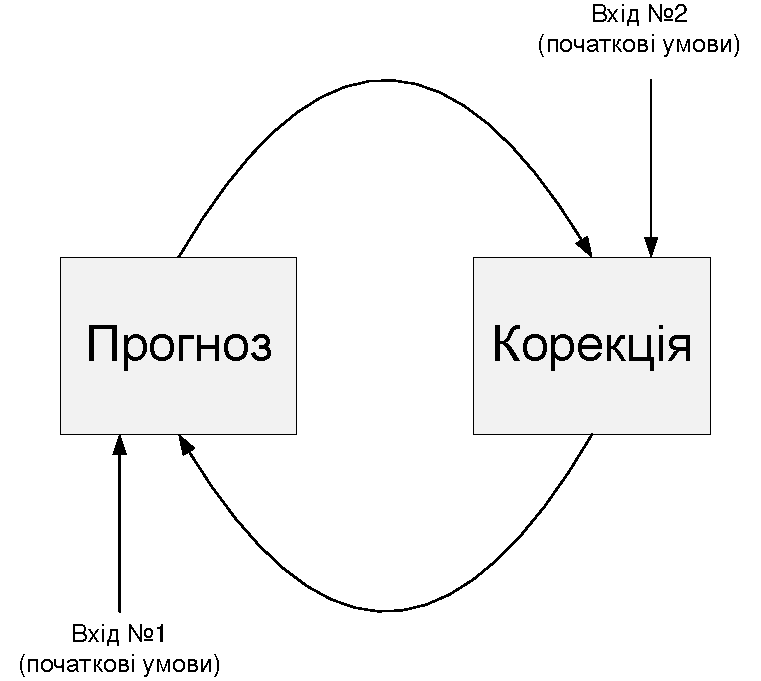
\includegraphics[scale=0.55]{pre_upd}
\caption{Цикл функціонування фільтра Калмана }
\label{fig:basic_cycle}
\end{figure} 



\begin{table}[here]
\small
\caption{Рівняння дискретного фільтра Калмана}
\centering
\begin{tabular}{|p{160mm}|} \hline 


Рівняння / Формула \\ \hline 
\begin{eqnarray} 
% \begin{array}{cc}
\text{Модель динаміки системи}  &  \label{eq:kalman_1} x_{k} = \Phi x_{k-1} + w_{k-1}, \\  
\text{Модель вимірювань}  & \label{eq:kalman_2} z_{k} = Hx_{k} +v_{k} \\ 
\text{Початкові умови}  &\label{eq:kalman_3} E[x_{o}] = \hat{x}_{0}, E[x_{o} x_{o}^{T}] = P_{0} \\
\text{Припущення незалежності}  &  \label{eq:kalman_4} E[w_{k} v_{j}^{T}] = 0 \text{для всіх k та j} \\
\text{Екстраполяція оцінки (прогноз)}  &  \label{eq:kalman_5} \hat{x}_{k}(-) = \Phi \hat{x}_{k-1}(+)\\
\text{Екстраполяція коваріації}  &  \label{eq:kalman_6} P_{k}(-) = \Phi_{k-1} P_{k-1}(+)\Phi_{k-1}^{T} + Q_{k-1} \\ 
\text{Корекція оцінки}  &  \label{eq:kalman_7} \hat{x}_{k}(+) = \hat{x}_{k}(-) + K_{k}[z_{k}-H_{k}\hat{x}_{k}(-)]\\
\text{Корекція оцінки коваріації}  &  \label{eq:kalman_8} P_{k}(+) = [I - K_{k}H_{k}]P_{k}(-)\\
\text{Коефіцієнт підсилення Калмана}   &  \label{eq:kalman_9} K_{k}= P_{k}(-)H_{k}^{T}[H_{k}P_{k}(-)H_{k}^{T} + R_{k}]^{-1}  
% \end{array}
\end{eqnarray} 
\\  \hline
\end{tabular}
\label{tb:ac}
\end{table}
Перше завдання при корекції -- розрахувати коефіцієнт підсилення Калмана, $K_{k}$/
Наступний крок, безпосередньо отримати виміри $z_{k}$, а потім генерувати 
апостеріорну оцінку за допомогою \eqref{eq:k_update}. Останній крок  -- це 
отримання апостеріорної коваріаційної матриці оцінки помилки.

Після кожного разу екстраполяції та корекції, процес повторюється, попередні
апостеріорні оцінки використовуються для прогнозу нових апріорних оцінок.
Ця рекурсивна природа є найбільш важливою особливістю фільтра Калмана, це робить
його більш практичним, в порівнянні з іншими фільтрами (наприклад фільтр Віннера)
\begin{figure}[here]
\centering
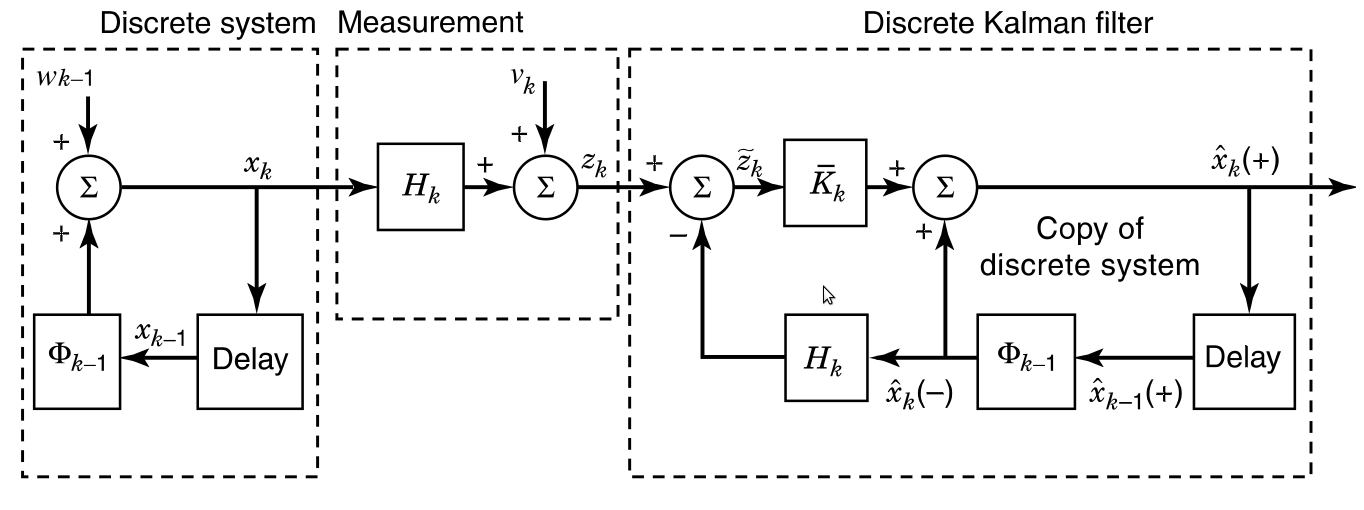
\includegraphics[scale=0.35]{kalman_flow}
\caption{Блок діаграма системи, моделі вимірювань та дискретного ФК}
\label{fig:kalman_flow}
\end{figure} 

\subsection{Проектування фільтра Калмана}

В практичній реалізації фільтра, коваріація вимірюваного шуму R вимірюється
звичайно до використання фільтра. Знаходження цієї матриці в загальному випадку
практична задача, виміряні величини дають можливість визначити дисперсію шуму, що
діє на данні датчиків.

Визначення коваріації шуму системи Q в загальному більш складна задача,
просто не має можливості безпосередньо спостерігати процес який оцінюється.
Інколи відносно проста модель процесу може дати прийнятний результат, якщо
введена достатня величина невизначеності процесу через вибір матриці Q.

В іншому випадку, є чи немає раціональної бази для вибору параметрів, часто
краща продуктивність (з точки зору статистики) може бути отримана за допомогою
налаштування параметрів фільтра Q та R. 

Асиметрія коваріаційної матриці $P$ один з факторів, що впливає на чисельну
нестійкість рівняння Рікатті. Якщо не використовується фільтр з квадратним
коренем, тоді ця матриця може бути ``симетризована'' просто за наступною 
формулою:
\begin{equation}
 \label{P_symetry}
P= \frac{1}{2}(P+P^{T})
\end{equation}
Цей метод використовується протягом довгого часу і добре себе зарекомендував.

При проектуванні фільтра, корекція коваріаційної матриці \eqref{eq:kalman_6} та
\eqref{eq:kalman_8} має бути перевірена не тільки на симетрію але й на 
додатно визначеність.
Якщо ці умови не будуть виконуються, це свідчить про помилки в програмі або
матриця погано обумовлена. Для усунення проблеми обумовленості використовується
інше рівняння для $P_{k}(+)$, яке називається формою Джозефа \cite{joseph}, яка показна на
наступному рівнянні:
\begin{equation}
 \label{P_plus_Joseph}
P_{k}(+)=[I-K_{k}H_{k}]P_{k}(-)[I-K_{k}H_{k}]^{T}+K_{k}R_{k}K_{k}^{T}
\end{equation}
З рівняння видно, що права частина є сумою двох симетричних матриць.
Перша додатно визначена інша не від'ємно визначена, що робить $P_{k}(+)$ 
додатно визначеною матрицею.

Безперечно саме фільтр Калмана найбільш привабливий при розв’язанні задачі 
комплексної обробки інформації в інерціально-супутникових системах навігації. 
Проте використання фільтра Калмана зустрічає певні труднощі при його практичної
 реалізації на борту ЛА. Зокрема в жорстко зв’язаних   інерціально-супутникових 
системах навігації,  фільтр Калмана повинний бути дуже швидкодіючим, що обмежується 
характеристиками існуючих процесорів бортових ЦОМ. 




